\documentclass[11pt, a4paper]{article}

% --- High Quality Classic Typography ---
\usepackage[utf8]{inputenc}
\usepackage[T1]{fontenc}
\usepackage{mathptmx}
\usepackage{microtype}
\usepackage{setspace}
\setstretch{1.15}

% --- Page Layout ---
\usepackage[margin=1in]{geometry}
\usepackage{fancyhdr}

% --- Graphics, Algorithms & Diagrams ---
\usepackage{graphicx}
\usepackage{booktabs}
\usepackage{caption}
\usepackage{float}
\usepackage[ruled,vlined]{algorithm2e}
\usepackage{tikz}
\usetikzlibrary{shapes.geometric, arrows, positioning, fit, calc}

% TikZ Styles
\tikzstyle{process} = [rectangle, minimum width=3cm, minimum height=1cm, text centered, draw=black, fill=blue!10, rounded corners]
\tikzstyle{database} = [cylinder, shape border rotate=90, draw, minimum height=1.5cm, minimum width=1.5cm, text centered, fill=orange!10]
\tikzstyle{actor} = [circle, draw, minimum size=1cm, text centered, fill=green!10]
\tikzstyle{arrow} = [thick,->,>=stealth]

% --- Syntax Highlighting ---
\usepackage{listings}
\usepackage{xcolor}
\definecolor{codegray}{rgb}{0.5,0.5,0.5}
\definecolor{codepurple}{rgb}{0.58,0,0.82}
\definecolor{backcolour}{rgb}{0.95,0.95,0.92}
\lstdefinestyle{mystyle}{
    backgroundcolor=\color{backcolour},   
    commentstyle=\color{codegray},
    keywordstyle=\color{magenta},
    numberstyle=\tiny\color{codegray},
    stringstyle=\color{codepurple},
    basicstyle=\ttfamily\footnotesize,
    breakatwhitespace=false,         
    breaklines=true,                 
    captionpos=b,                    
    keepspaces=true,                 
    numbers=left,                    
    numbersep=5pt,                  
    showspaces=false,                
    showstringspaces=false,
    showtabs=false,                  
    tabsize=2
}
\lstset{style=mystyle}

% --- Links & Metadata ---
\usepackage[colorlinks=true, linkcolor=black, citecolor=blue, urlcolor=blue]{hyperref}

% --- Header & Footer Setup ---
\pagestyle{fancy}
\fancyhf{}
\lhead{\textit{JournaBuddy Research Report}}
\rhead{\thepage}
\renewcommand{\headrulewidth}{0.4pt}

% --- Title Page Info ---
\title{\textbf{\Huge Development and Architectural Report}\\[0.5em]
\Large JournaBuddy: A Multi-Agent AI Research Intelligence Platform}

\author{
    \textbf{Abdullah Al Mamun} \\
    \textit{B.Sc. Software Engineering, Daffodil International University} \\
    \textit{M.Sc. Software Engineering (in progress), TU Wien} \\
    \href{mailto:mamun.swe.de@gmail.com}{mamun.swe.de@gmail.com} \\
    ORCID: \href{https://orcid.org/0009-0006-7473-0024}{0009-0006-7473-0024}
}
\date{\today}

\begin{document}

\maketitle
\thispagestyle{empty} 

\begin{abstract}
The peer-review and pre-submission evaluation phase of academic publishing is historically bottlenecked by manual review processes, citation verification, and rigorous plagiarism checks. This report details the full development lifecycle, architectural design, and algorithmic implementation of \textbf{JournaBuddy}, an advanced AI-powered research intelligence platform. 
\end{abstract}

\tableofcontents
\newpage

\section{System Architecture and Flow}

\subsection{Use Case Diagram}
Figure \ref{fig:usecase} illustrates the core interactions between the Researcher and the JournaBuddy ecosystem.

\begin{figure}[H]
\centering
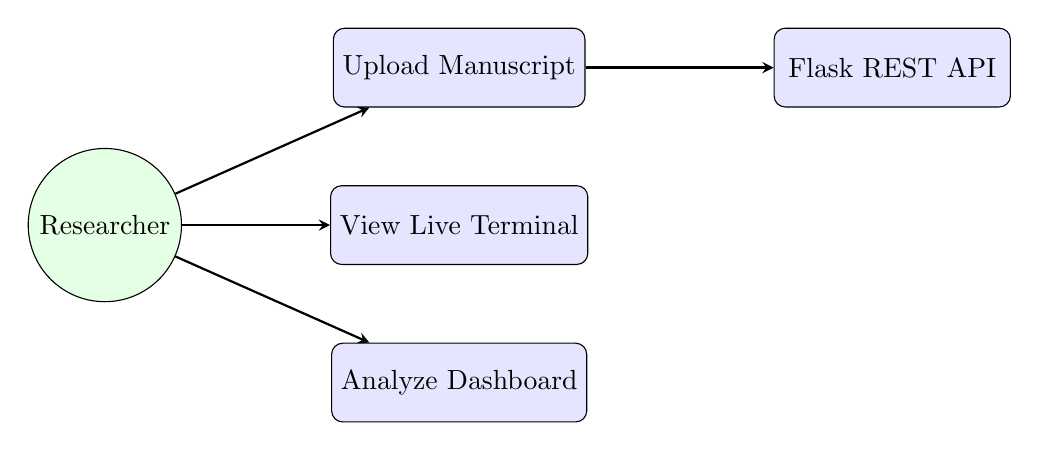
\begin{tikzpicture}[node distance=2.5cm]
    \node (user) [actor] {Researcher};
    \node (upload) [process, right of=user, xshift=2cm, yshift=2cm] {Upload Manuscript};
    \node (view) [process, right of=user, xshift=2cm, yshift=0cm] {View Live Terminal};
    \node (dashboard) [process, right of=user, xshift=2cm, yshift=-2cm] {Analyze Dashboard};
    
    \node (api) [process, right of=upload, xshift=3cm] {Flask REST API};
    
    \draw [arrow] (user) -- (upload);
    \draw [arrow] (user) -- (view);
    \draw [arrow] (user) -- (dashboard);
    \draw [arrow] (upload) -- (api);
\end{tikzpicture}
\caption{System Use Case Diagram}
\label{fig:usecase}
\end{figure}

\subsection{System Flowchart}
Figure \ref{fig:flowchart} outlines the asynchronous data flow from upload to final BI rendering.

\begin{figure}[H]
\centering
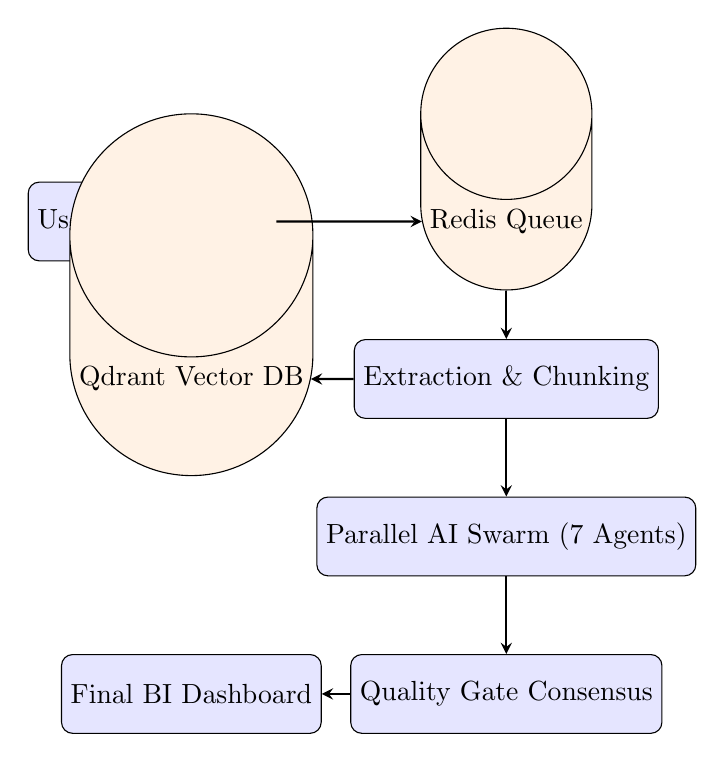
\begin{tikzpicture}[node distance=2cm]
    \node (start) [process] {User Uploads PDF};
    \node (redis) [database, right of=start, xshift=2.5cm] {Redis Queue};
    \node (extract) [process, below of=redis] {Extraction \& Chunking};
    \node (parallel) [process, below of=extract] {Parallel AI Swarm (7 Agents)};
    \node (qdrant) [database, left of=extract, xshift=-2cm] {Qdrant Vector DB};
    \node (gate) [process, below of=parallel] {Quality Gate Consensus};
    \node (dash) [process, left of=gate, xshift=-2cm] {Final BI Dashboard};
    
    \draw [arrow] (start) -- (redis);
    \draw [arrow] (redis) -- (extract);
    \draw [arrow] (extract) -- (qdrant);
    \draw [arrow] (extract) -- (parallel);
    \draw [arrow] (parallel) -- (gate);
    \draw [arrow] (gate) -- (dash);
\end{tikzpicture}
\caption{Asynchronous Pipeline Flowchart}
\label{fig:flowchart}
\end{figure}

\section{Core Algorithms}

\subsection{Robust LLM JSON Extraction Algorithm}
To handle unstructured conversational output from Large Language Models (LLMs), a two-step fallback algorithm (Algorithm \ref{algo:json}) was engineered.

\begin{lstlisting}[language=Python, caption=Robust Two-Step JSON Extraction Fallback, label=algo:json]
def extract_json(raw_response):
    # Step 1: Regex Block Extraction
    if contains_markdown_blocks(raw_response):
        extracted = regex_extract_backticks(raw_response)
        return json.loads(extracted)
        
    # Step 2: Bracket Parsing Fallback
    else:
        start_idx = raw_response.find('{')
        end_idx = raw_response.rfind('}')
        sliced = raw_response[start_idx : end_idx + 1]
        return json.loads(sliced)
\end{lstlisting}

\section{Parallel Agent Implementation}
The system utilizes a Thread Pool Executor to run independent AI agents simultaneously, as visualized in Figure \ref{fig:swarm}. This significantly reduces the inference latency.

\begin{figure}[H]
\centering
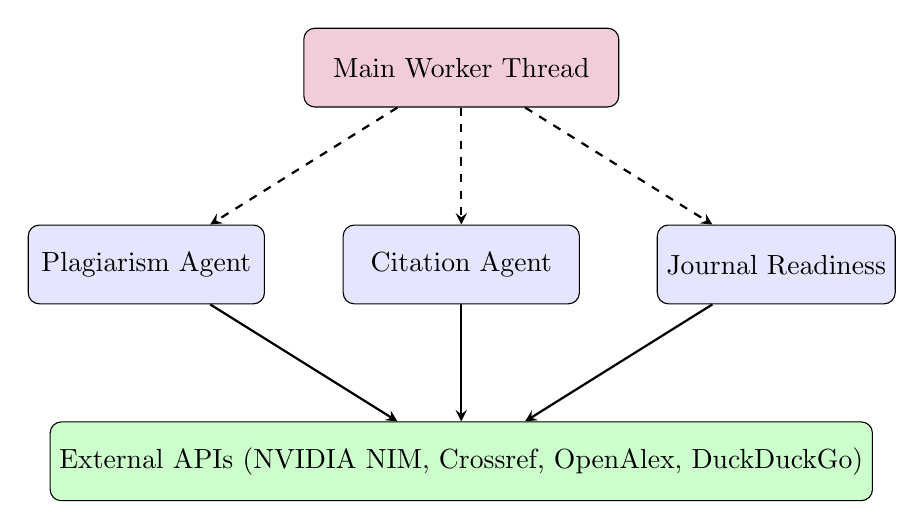
\begin{tikzpicture}[node distance=1.5cm]
    \node (main) [process, fill=purple!20, minimum width=4cm] {Main Worker Thread};
    
    \node (a1) [process, below of=main, xshift=-4cm, yshift=-1cm] {Plagiarism Agent};
    \node (a2) [process, below of=main, xshift=0cm, yshift=-1cm] {Citation Agent};
    \node (a3) [process, below of=main, xshift=4cm, yshift=-1cm] {Journal Readiness};
    
    \node (apis) [process, fill=green!20, below of=a2, yshift=-1cm, minimum width=10cm] {External APIs (NVIDIA NIM, Crossref, OpenAlex, DuckDuckGo)};
    
    \draw [arrow, dashed] (main) -- (a1);
    \draw [arrow, dashed] (main) -- (a2);
    \draw [arrow, dashed] (main) -- (a3);
    
    \draw [arrow] (a1) -- (apis);
    \draw [arrow] (a2) -- (apis);
    \draw [arrow] (a3) -- (apis);
\end{tikzpicture}
\caption{Concurrent Multi-Agent Swarm Architecture}
\label{fig:swarm}
\end{figure}

\section{Conclusion}
JournaBuddy integrates complex NLP algorithms, real-time API integrations, and robust concurrency mechanisms to deliver a state-of-the-art pre-submission screening tool. 

\end{document}
